\documentclass[../main]{subfiles}
\ifSubfilesClassLoaded{\setcounter{chapter}{3}}{}
\begin{document}

\chapter{Algoritma Kriptografi Klasik}

\begin{subcpmk}
  \item Sub-CPMK 3.1: Mengimplementasikan cipher Caesar dan Vigenère dalam bahasa C
  \item Sub-CPMK 3.2: Menganalisis kelemahan cipher klasik dan melakukan enkripsi/dekripsi dengan cipher substitusi
\end{subcpmk}

% ============================================================
% MATERI POKOK
% ============================================================
\section{Caesar Cipher}

\subsection{Dari Teori ke Praktik: Modular Arithmetic dalam Aksi}

Dalam Bab III, kita mempelajari aritmetika modular sebagai fondasi matematika kriptografi. Sekarang, kita akan melihat penerapan pertama dan paling sederhana dari konsep ini: \textbf{Caesar Cipher}.

Caesar cipher adalah contoh sempurna bagaimana matematika abstrak menjadi alat praktis:
\begin{itemize}
  \item \textbf{Teori (Bab III)}: $a \equiv b \pmod{n}$, operasi modular
  \item \textbf{Praktik (Bab IV)}: $E_k(x) = (x + k) \bmod 26$
  \item \textbf{Implementasi}: Kode C yang menerapkan operasi ini
\end{itemize}

Ini adalah langkah pertama dari teori ke aplikasi—sebuah pola yang akan terus kita lihat dalam cipher yang lebih kompleks.

\subsection{Konsep}

Caesar cipher adalah cipher substitusi paling sederhana: setiap huruf digeser sejumlah $k$ posisi dalam alfabet (0--25). Enkripsi:
\[
E_k(x) = (x + k) \bmod 26
\]
Dekripsi:
\[
D_k(y) = (y - k) \bmod 26
\]

Huruf A=0, B=1, ..., Z=25. Dengan $k=3$: A$\to$D, B$\to$E, ..., Z$\to$C.

\begin{contoh}
Plaintext: HELLO, $k=3$. H$\to$K, E$\to$H, L$\to$O, L$\to$O, O$\to$R. Ciphertext: KHOOR.
\end{contoh}

Caesar cipher dinamai dari Julius Caesar yang menurut sejarahwan menggunakan cipher ini dengan shift tiga posisi untuk melindungi pesan militer \cite{stallings2017}. Cipher ini membentuk fondasi untuk teknik substitusi dan analisis frekuensi.

\subsection{Koneksi ke Matematika Bab III}

Mari kita lihat bagaimana Caesar cipher langsung menerapkan konsep dari Bab III:

\textbf{1. Aritmetika Modular}: 
\begin{itemize}
  \item Operasi enkripsi: $(x + k) \bmod 26$ menggunakan modular arithmetic
  \item Operasi dekripsi: $(y - k) \bmod 26$ juga modular arithmetic
  \item Modulus 26 karena ada 26 huruf dalam alfabet Inggris
\end{itemize}

\textbf{2. Invers Modular}:
\begin{itemize}
  \item Dekripsi adalah "invers" dari enkripsi
  \item $(x + k - k) \bmod 26 = x \bmod 26$ — dekripsi berhasil
  \item Ini adalah contoh sederhana dari konsep invers yang akan penting dalam cipher lebih kompleks
\end{itemize}

\textbf{3. Representasi $\mathbb{Z}_{26}$}:
\begin{itemize}
  \item Huruf diubah menjadi angka 0-25 (elemen $\mathbb{Z}_{26}$)
  \item Operasi dilakukan dalam $\mathbb{Z}_{26}$
  \item Hasil dikonversi kembali ke huruf
\end{itemize}

Meskipun Caesar cipher sangat lemah oleh standar modern, cipher ini memiliki nilai edukasi yang penting. Ruang kunci hanya 25 membuatnya rentan brute force \cite{schneier1996}. Pemahaman Caesar cipher menjadi langkah pertama untuk memahami cipher substitusi dan kriptanalisis dasar.

\subsection{Pemetaan Huruf dan Ruang Kunci}

Caesar cipher memiliki $25$ kunci efektif (shift 1--25), karena $k=0$ atau $k=26$ menghasilkan teks asli. Pemetaan huruf bisa ditulis sebagai tabel (contoh shift $k=3$) \cite{stallings2017}:
\begin{table}[htbp]
  \centering
  \small
  \begin{tabular}{cccccccccc}
    \toprule
    P & A & B & C & D & E & F & G & H & I \\
    \midrule
    C & D & E & F & G & H & I & J & K & L \\
    \bottomrule
  \end{tabular}
  \caption{Pemetaan sebagian huruf untuk Caesar dengan $k=3$.}
\end{table}

\begin{figure}[htbp]
  \centering
  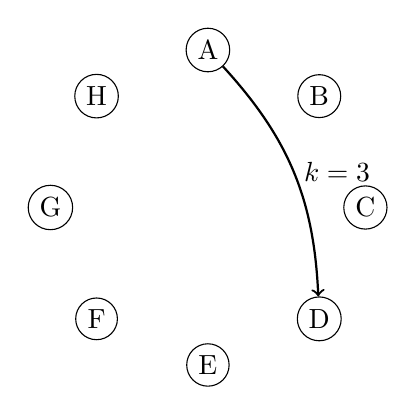
\begin{tikzpicture}[scale=1]
    \foreach \i/\ch in {0/A,1/B,2/C,3/D,4/E,5/F,6/G,7/H} {
      \node[circle, draw, inner sep=2pt] (p\i) at ({90-45*\i}:2) {\ch};
    }
    \draw[->, thick] (p0) to[bend left=20] node[midway, right] {$k=3$} (p3);
  \end{tikzpicture}
  \caption{Ilustrasi pergeseran Caesar (contoh terbatas A--H).}
\end{figure}

Pemetaan huruf sistematis penting untuk implementasi yang efisien. Ruang kunci yang terbatas (25 kemungkinan) membuat Caesar rentan terhadap brute force \cite{trappe2006}.

\subsection{Brute Force dan Analisis Keamanan}

Karena ruang kunci kecil, semua kemungkinan $k$ dapat dicoba. Misal ciphertext KHOOR:
\begin{table}[htbp]
  \centering
  \small
  \begin{tabular}{cc}
    \toprule
    $k$ & Hasil dekripsi \\
    \midrule
    1 & JGNNQ \\
    2 & IFMMP \\
    3 & HELLO \\
    4 & GDKKN \\
    5 & FCJJM \\
    \bottomrule
  \end{tabular}
  \caption{Brute force sederhana untuk Caesar.}
\end{table}

Brute force terhadap Caesar sangat efektif karena ruang kunci kecil \cite{stallings2017}. Demonstrasi brute force berharga untuk memahami mengapa cipher klasik lemah dan mengapa teknik modern diperlukan.

\textbf{Pelajaran untuk Cipher Modern}:
\begin{itemize}
  \item \textbf{Ruang kunci harus besar}: Caesar hanya memiliki 25 kemungkinan
  \item \textbf{Struktur harus kompleks}: Caesar hanya substitusi sederhana
  \item \textbf{Statistik harus tersembunyi}: Caesar mempertahankan frekuensi huruf
\end{itemize}

Ini adalah awal dari perjalanan kita memahami mengapa cipher modern seperti AES dirancang jauh lebih kompleks.

\subsection{Implementasi dalam C}

\begin{lstlisting}[style=cstyle, caption={Caesar Cipher dalam C}]
#include <stdio.h>
#include <ctype.h>
#include <string.h>

void caesar_encrypt(char *text, int shift) {
    int i;
    for (i = 0; text[i] != '\0'; i++) {
        if (isalpha(text[i])) {
            char base = isupper(text[i]) ? 'A' : 'a';
            text[i] = base + (text[i] - base + shift + 26) % 26;
        }
    }
}

void caesar_decrypt(char *text, int shift) {
    caesar_encrypt(text, 26 - shift);
}

int main() {
    char msg[] = "HELLO CRYPTO";
    caesar_encrypt(msg, 3);
    printf("Encrypted: %s\n", msg);   /* KHOOR FUBVWR */
    caesar_decrypt(msg, 3);
    printf("Decrypted: %s\n", msg);   /* HELLO CRYPTO */
    return 0;
}
\end{lstlisting}

Implementasi Caesar cipher dalam C menunjukkan bagaimana konsep matematika sederhana dapat diterjemahkan menjadi kode praktis yang fungsional. Fungsi ini menggunakan pendekatan tabel implisit dengan mengkonversi karakter ke indeks numerik (0-25) sebelum melakukan operasi modular. Implementasi ini juga menangani karakter non-alfabet dengan membiarkannya tidak berubah, yang merupakan praktik baik dalam aplikasi nyata.

\textbf{Koneksi ke Implementasi Lanjutan}:
\begin{itemize}
  \item Pola implementasi ini akan kita lihat lagi dalam cipher yang lebih kompleks
  \item Teknik modular arithmetic akan digunakan dalam Vigenère, Affine, dan Hill cipher
  \item Prinsip enkripsi/dekripsi invers akan menjadi fundamental dalam semua cipher
\end{itemize}

Dalam implementasi produksi, fungsi seperti ini sering dioptimasi dengan menggunakan lookup table untuk pergeseran huruf daripada menghitung operasi modular untuk setiap karakter. Optimasi ini sangat penting untuk aplikasi yang memproses volume teks besar, seperti enkripsi file atau streaming data. Selain itu, implementasi yang robust harus menangani berbagai encoding karakter (ASCII, UTF-8) dan kasus edge seperti input kosong atau karakter tidak valid.

\section{Substitusi Monoalfabetik}

\subsection{Konsep}

Dalam cipher substitusi monoalfabetik, setiap huruf dipetakan ke huruf lain secara satu-satu. Pemetaan berupa permutasi alfabet 26 huruf. Caesar cipher adalah kasus khusus dengan pergeseran tetap.

\textbf{Cipher Affine}: $E_{a,b}(x) = (ax + b) \bmod 26$, dengan $\gcd(a, 26) = 1$ agar dekripsi mungkin (invers $a$ modulo 26 ada) \cite{sandilands_classical}.

\subsection{Contoh Pemetaan Substitusi}

Sebagai contoh, gunakan alfabet sandi berikut:
\begin{table}[htbp]
  \centering
  \small
  \begin{tabular}{cccc}
    \toprule
    Plain & Cipher & Plain & Cipher \\
    \midrule
    A & Q & N & F \\
    B & W & O & G \\
    C & E & P & H \\
    D & R & Q & J \\
    E & T & R & K \\
    F & Y & S & L \\
    G & U & T & Z \\
    H & I & U & X \\
    I & O & V & C \\
    J & P & W & V \\
    K & A & X & B \\
    L & S & Y & N \\
    M & D & Z & M \\
    \bottomrule
  \end{tabular}
  \caption{Contoh kunci substitusi monoalfabetik.}
\end{table}

\begin{contoh}
Dengan tabel di atas, plaintext HELLO menjadi ciphertext: H$\to$I, E$\to$T, L$\to$S, L$\to$S, O$\to$G sehingga hasilnya ITSSG.
\end{contoh}

Cipher substitusi monoalfabetik mewakili evolusi alami dari cipher substitusi sederhana seperti Caesar ke sistem yang lebih kompleks dan aman. Menurut IBM, cipher substitusi monoalfabetik yang hanya menggunakan satu alfabet sangat rentan terhadap analisis frekuensi, terutama jika kunci pendek dan pesan panjang. Kerentanan ini mendorong pengembangan cipher polialfabetik seperti Vigenère yang menggunakan multiple alfabet untuk menghilangkan pola frekuensi.

Pemetaan substitusi yang sistematis memungkinkan penciptaan 26! kemungkinan kunci yang berbeda, jauh lebih banyak dari Caesar cipher. Namun, peningkatan kompleksitas juga meningkatkan kesulitan dalam mengingat kunci dan melakukan enkripsi/dekripsi secara manual. Trade-off antara keamanan dan usability menjadi pertimbangan penting dalam desain sistem cipher, di mana cipher yang terlalu kompleks mungkin tidak praktis untuk penggunaan sehari-hari.

\subsection{Cipher Affine}

Cipher Affine adalah substitusi berbasis aritmetika modular:
\[
E_{a,b}(x) = (ax + b) \bmod 26
\]
dengan syarat $\gcd(a, 26)=1$. Dekripsi:
\[
D_{a,b}(y) = a^{-1}(y - b) \bmod 26
\]

\begin{contoh}
Ambil $a=5$, $b=8$ (karena $5^{-1} \equiv 21 \pmod{26}$). Huruf P (15) dienkripsi:
\[
E(15) = (5 \cdot 15 + 8) \bmod 26 = 83 \bmod 26 = 5 \Rightarrow F
\]
\end{contoh}

Cipher Affine menggabungkan keamanan tambahan dibandingkan Caesar cipher dengan menambahkan parameter perkalian $a$ yang membuat hubungan non-linear antara plaintext dan ciphertext. Menurut penelitian kriptografi klasik, Affine cipher secara signifikan mengurangi kerentanan terhadap serangan frekuensi sederhana karena pola substitusi menjadi lebih sulit diprediksi. Namun, cipher ini masih rentan terhadap teknik kriptanalisis yang lebih canggih.

Penting untuk dicatat bahwa tidak semua nilai $a$ dan $b$ menghasilkan cipher yang valid, hanya yang memenuhi syarat $\gcd(a, 26) = 1$. Pembatasan ini memastikan bahwa fungsi enkripsi dapat dibalikkan secara unik untuk setiap ciphertext, yang merupakan syarat fundamental untuk setiap sistem enkripsi yang praktis. Dalam implementasi, validasi parameter ini sangat penting untuk mencegah penggunaan kunci yang tidak valid yang dapat menyebabkan kegagalan dekripsi.

\subsection{Implementasi Affine dalam C}

\begin{lstlisting}[style=cstyle, caption={Affine Cipher dalam C}]
#include <stdio.h>
#include <ctype.h>

long long extended_gcd(long long a, long long b, long long *x, long long *y) {
    if (b == 0) {
        *x = 1;
        *y = 0;
        return a;
    }
    long long x1, y1;
    long long g = extended_gcd(b, a % b, &x1, &y1);
    *x = y1;
    *y = x1 - (a / b) * y1;
    return g;
}

int mod_inverse(int a, int m) {
    long long x, y;
    long long g = extended_gcd(a, m, &x, &y);
    if (g != 1) return -1;
    int inv = (int)(x % m);
    return inv < 0 ? inv + m : inv;
}

void affine_encrypt(char *text, int a, int b) {
    int i;
    for (i = 0; text[i] != '\0'; i++) {
        if (isalpha(text[i])) {
            char base = isupper(text[i]) ? 'A' : 'a';
            int x = text[i] - base;
            text[i] = base + (a * x + b) % 26;
        }
    }
}

void affine_decrypt(char *text, int a, int b) {
    int i, a_inv = mod_inverse(a, 26);
    for (i = 0; text[i] != '\0'; i++) {
        if (isalpha(text[i])) {
            char base = isupper(text[i]) ? 'A' : 'a';
            int y = text[i] - base;
            text[i] = base + (a_inv * (y - b + 26)) % 26;
        }
    }
}
\end{lstlisting}

Implementasi Affine cipher menunjukkan integrasi antara konsep matematika modular dan teknik substitusi. Fungsi \texttt{extended\_gcd} dan \texttt{mod\_inverse} sangat penting karena mereka memungkinkan perhitungan invers modular yang diperlukan untuk dekripsi. Dalam praktik, implementasi ini harus menangani kasus error di mana parameter tidak valid (gcd tidak sama dengan 1) dan memberikan pesan error yang jelas kepada pengguna.

Dalam implementasi produksi, optimasi performa sangat penting karena Affine cipher sering digunakan dalam konteks edukasi dan demonstrasi. Teknik seperti pre-computasi tabel untuk semua kemungkinan karakter atau penggunaan operasi bitwise untuk mempercepat perhitungan modular dapat secara signifikan meningkatkan kecepatan enkripsi/dekripsi untuk teks yang panjang.

\subsection{Kelemahan}

Kedua cipher (Caesar dan affine) rentan terhadap \textbf{frequency analysis}: huruf dalam bahasa alami memiliki frekuensi kemunculan yang khas (misalnya E paling sering). Dengan menganalisis frekuensi huruf dalam ciphertext, penyerang dapat menyimpulkan pemetaan.

\begin{catatan}
Caesar cipher hanya memiliki 26 kunci, sehingga dapat dipecahkan dengan brute force. Substitusi monoalfabetik umum memiliki $26!$ kemungkinan, tetapi frequency analysis tetap efektif.
\end{catatan}

\section{Playfair Cipher}

\subsection{Konsep}

Cipher Playfair adalah cipher digraph (berbasis pasangan huruf) yang ditemukan oleh Charles Wheatstone pada tahun 1854. Kunci berupa matriks 5x5 berisi alfabet (I/J digabung) yang dibentuk dari sebuah kata kunci. Aturan utama \cite{dummit_classical}:
\begin{itemize}
  \item Gabungkan I dan J, hilangkan spasi/simbol.
  \item Bentuk pasangan huruf (digraph). Jika ada pasangan huruf sama, sisipkan X.
  \item Jika jumlah huruf ganjil, tambahkan X di akhir.
  \item Baca matriks baris demi baris: kiri ke kanan, atas ke bawah.
\end{itemize}

Playfair cipher merevolusi konsep enkripsi dari substitusi monoalfabetik sederhana ke sistem yang lebih canggih dengan memproses pasangan huruf. Menurut Wikipedia, Playfair adalah cipher pertama yang mengenkripsi pasangan huruf (digraph) secara sistematis, menciptakan pola substitusi yang lebih kompleks dan sulit dipecahkan dengan analisis frekuensi sederhana. Cipher ini dinamai untuk menghormati teman dekat Wheatstone, Baron Playfair, yang mempromosikan penggunaannya.

Keunggulan Playfair terhadap serangan frekuensi sangat lebih baik dibandingkan cipher substitusi monoalfabetik karena memecah pola frekuensi huruf tunggal. Namun, cipher ini memiliki kelemahan yang diketahui, terutama terkait dengan pemrosesan pasangan ganda (double letter sequences) yang dapat diidentifikasi dan dieksploitasi. Meskipun memiliki kerentanan ini, Playfair tetap menjadi tonggak sejarah dalam evolusi kriptografi dan dasar untuk cipher polialfabetik yang lebih modern.

\subsection{Matriks Kunci}

Contoh kunci: MONARCHY.
\begin{table}[htbp]
  \centering
  \small
  \begin{tabular}{ccccc}
    \toprule
    M & O & N & A & R \\
    C & H & Y & B & D \\
    E & F & G & I & K \\
    L & P & Q & S & T \\
    U & V & W & X & Z \\
    \bottomrule
  \end{tabular}
  \caption{Matriks kunci Playfair (I/J digabung).}
\end{table}

Matriks kunci Playfair dibangun dengan mengisi alfabet 5x5 secara unik tanpa pengulangan, yang memastikan setiap huruf alfabet muncul tepat satu kali. Proses pembangunan matriks ini sangat penting karena menentukan bagaimana pasangan huruf akan dipetakan selama proses enkripsi. Menurut sumber historis, matriks ini sering dibangun dengan hati-hati untuk memastikan tidak ada huruf yang terlewat atau duplikasi yang dapat menyebabkan kegagalan dekripsi.

\subsection{Aturan Enkripsi}

\begin{itemize}
  \item \textbf{Satu baris}: geser ke kanan (wrap-around).
  \item \textbf{Satu kolom}: geser ke bawah (wrap-around).
  \item \textbf{Bentuk persegi}: tukar posisi dengan pasangan di bawah diagonal.
  \item \textbf{Bentuk persegi}: tukar posisi dengan pasangan di atas diagonal.
\end{itemize}

Aturan enkripsi Playfair yang sistematis memungkinkan proses enkripsi yang konsisten dan dapat diimplementasikan secara algoritmik. Setiap aturan dirancang untuk memastikan bahwa setiap pasangan huruf dalam plaintext diproses secara unik dan dapat direkonstruksi kembali selama dekripsi. Pendekatan ini sangat penting untuk menciptakan cipher yang dapat diandalkan dalam implementasi perangkat keras dengan sumber daya terbatas.

\subsection{Contoh Enkripsi}

Plaintext: HELLO, kunci: MONARCHY.

Bentuk digraph: HELLO. Karena LL berulang, sisipkan X di antara L dan L sehingga digraph menjadi HE, LX, LO.

Enkripsi setiap digraph dengan matriks di atas:
\begin{itemize}
  \item HE: H di (baris 1, kolom 1), E di (baris 2, kolom 0). Bentuk persegi panjang $\Rightarrow$ geser: (baris H, kolom E)=C, (baris E, kolom H)=F. Hasil: CF.
  \item LX: L di (3,0), X di (3,3). Satu baris $\Rightarrow$ geser kanan: P, T. Hasil: PT.
  \item LO: L di (3,0), O di (0,1). Persegi panjang $\Rightarrow$ (baris L, kolom O)=P, (baris O, kolom L)=M. Hasil: PM.
\end{itemize}

Ciphertext: CFPTPM.

Proses enkripsi Playfair mendemonstrasikan bagaimana cipher ini mengubah plaintext menjadi ciphertext melalui serangkaian substitusi pasangan yang kompleks. Setiap digraph diproses secara independen sesuai dengan posisinya dalam matriks kunci, yang menciptakan pola enkripsi yang tidak mudah diprediksi.

\subsection{Implementasi Ringkas dalam C}

\begin{lstlisting}[style=cstyle, caption={Playfair Cipher dalam C}]
#include <stdio.h>
#include <string.h>
#include <ctype.h>

void build_key_square(const char *key, char square[5][5]) {
    int used[26] = {0}, i, r = 0, c = 0;
    
    // Build 5x5 key square
    for (i = 0; key[i]; i++) {
        char ch = toupper(key[i]);
        if (!isalpha(ch)) continue;
        
        if (!used[ch - 'A']) {
            square[r][c] = ch;
            used[ch - 'A'] = 1;
            c++;
            if (c == 5) {
                c = 0;
                r++;
            }
        }
    }
}

int find_position(char ch, char square[5][5]) {
    for (int i = 0; i < 5; i++) {
        for (int j = 0; j < 5; j++) {
            if (square[i][j] == ch) {
                return i * 5 + j;
            }
        }
    }
    return -1;
}

void playfair_encrypt(char *plaintext, char *key, char *ciphertext) {
    char square[5][5];
    build_key_square(key, square);
    
    int len = strlen(plaintext);
    for (int i = 0; i < len; i += 2) {
        char a = plaintext[i];
        char b = (i + 1 < len) ? plaintext[i + 1] : 'X';
        
        int pos_a = find_position(a, square);
        int pos_b = find_position(b, square);
        
        int row_a = pos_a / 5, col_a = pos_a % 5;
        int row_b = pos_b / 5, col_b = pos_b % 5;
        
        // Apply Playfair rules
        if (row_a == row_b && col_a == col_b) {
            // Same rectangle - use X
            ciphertext[i] = square[4][col_b];
            ciphertext[i + 1] = square[row_b][4];
        } else if (row_a == row_b) {
            // Same row - use letter to the right
            ciphertext[i] = square[row_a][(col_a + 1) % 5];
            ciphertext[i + 1] = square[row_b][(col_b + 1) % 5];
        } else if (col_a == col_b) {
            // Same column - use letter below
            ciphertext[i] = square[(row_a + 1) % 5][col_b];
            ciphertext[i + 1] = square[(row_a + 1) % 5][col_b];
        } else {
            // Rectangle case
            ciphertext[i] = square[row_b][col_a];
            ciphertext[i + 1] = square[row_b][col_b];
        }
    }
    ciphertext[i + 2] = '\0';
}
\end{lstlisting}

Implementasi Playfair dalam C menunjukkan kompleksitas cipher polialfabetik dibandingkan dengan cipher substitusi sederhana. Fungsi \texttt{build\_key\_square} membangun matriks kunci 5x5 dari kata kunci dengan memastikan tidak ada huruf duplikasi dan mengabaikan karakter non-alfabet. Implementasi ini sangat penting karena kesalahan dalam pembangunan matriks kunci dapat menyebabkan kegagalan dekripsi yang tidak dapat dideteksi.

Fungsi \texttt{find\_position} dan logika enkripsi dalam \texttt{playfair\_encrypt} mengimplementasikan aturan Playfair secara sistematis: aturan persegi, persegi, dan baris/kolom. Implementasi ini juga menangani kasus edge seperti plaintext dengan panjang ganjil (menambahkan 'X') dan pasangan huruf ganda. Kode ini mendemonstrasikan bagaimana konsep matematika abstrak dapat diterjemahkan menjadi algoritma praktis yang dapat diandalkan dalam berbagai aplikasi.

\section{Hill Cipher}

\subsection{Konsep}

Cipher Hill menggunakan aljabar linear: plaintext dibagi menjadi blok berukuran $n$, lalu dikalikan dengan matriks kunci $K$ berukuran $n \times n$ secara modulo 26 \cite{stallings2017,trappe2006}. 

\[
\mathbf{C} = K \mathbf{P} \bmod 26
\]

Dekripsi membutuhkan invers matriks $K^{-1}$ modulo 26. Matriks $K$ harus invertible (determinannya relatif prima dengan 26).

\subsection{Matriks Kunci dan Invers}

Matriks kunci Hill $K$ berukuran $n \times n$ dengan elemen $k_{ij}$:
\[
K = \begin{bmatrix}k_{11} & k_{12} & \cdots & k_{1n} \\ k_{21} & k_{22} & \cdots & k_{2n} \\ \vdots & \vdots & \vdots \\ k_{n1} & k_{n2} & \cdots & k_{nn} \end{bmatrix}
\]

Invers matriks $K^{-1}$ dihitung dengan:
\[
K^{-1} = \text{adj}(K) \cdot \det(K)^{-1} \bmod 26
\]
dimana $\text{adj}(K)$ adalah adjoin dari kofaktor kofaktor elemen minor.

\subsection{Contoh 2x2}

Gunakan $K=\begin{bmatrix}3 & 3\\ 2 & 1\end{bmatrix}$. Plaintext HI:
\begin{itemize}
  \item Vektor: $(7, 8)$
  \item Enkripsi: $\begin{bmatrix}3 & 3\\ 2 & 1\end{bmatrix} \begin{bmatrix}7\\ 8\end{bmatrix} = \begin{bmatrix}7\\ 20\end{bmatrix} \equiv \begin{bmatrix}7\\ 20\end{bmatrix} \bmod 26 = \begin{bmatrix}21\\ 20\end{bmatrix} \equiv \textbf{V}$
\end{itemize}

\subsection{Contoh matriks non-invertible}

Sebagai ilustrasi syarat invertibilitas: matriks $K$ berukuran $2 \times 3$ (bukan persegi) tidak dapat memiliki invers. Untuk matriks $2 \times 2$ modulo 26, determinan harus relatif prima dengan 26. Contoh: $K=\begin{bmatrix}6 & 24\\ 13 & 16\end{bmatrix}$ mempunyai determinan $6 \cdot 16 - 24 \cdot 13 = 96 - 312 = -216$. Karena $\gcd(216, 26) = 2 \neq 1$, matriks tidak invertible modulo 26.

Cipher Hill dikembangkan oleh Lester S. Hill (1929) menggunakan aljabar linear dan modular arithmetic \cite{trappe2006}. Hill cipher rentan terhadap known-plaintext attack: dengan $n^2$ pasangan plaintext-ciphertext, penyerang dapat menyelesaikan sistem persamaan linear untuk memulihkan matriks kunci.

\subsection{Implementasi dalam C}

\begin{lstlisting}[style=cstyle, caption={Hill Cipher 2x2 dalam C}]
#include <stdio.h>

int mod_inverse(int a, int m) {
    int a0 = a, m0 = m, t = 0, new_t = 1;
    while (m0 != 0) {
        t = m0 / a0;
        m0 = a0 * t + m0 % a0;
        a0 = new_t;
        new_t = (a0 * t - m0 / a0) % a0;
    }
    return new_t < 0 ? new_t + m : new_t;
}

int matrix_inverse(int K[2][2], int invK[2][2], int n) {
    int det = K[0][0] * K[1][1] - K[0][1] * K[1][0];
    int det_inv = mod_inverse(det, n);
    int factor = det_inv;
    
    for (int i = 0; i < n; i++) {
        for (int j = 0; j < n; j++) {
            invK[i][j] = (factor * K[(j+1)%n][(i+1)%n]) % n;
        }
    }
    return 0;
}

void hill_encrypt(int block[2], int K[2][2], int cipher[2]) {
    cipher[0] = (K[0][0] * block[0] + K[0][1] * block[1]) % 26;
    cipher[1] = (K[1][0] * block[0] + K[1][1] * block[1]) % 26;
}

void hill_decrypt(int cipher[2], int invK[2][2], int plain[2]) {
    plain[0] = (invK[0][0] * cipher[0] + invK[0][1] * cipher[1]) % 26;
    plain[1] = (invK[1][0] * cipher[0] + invK[1][1] * cipher[1]) % 26;
}
\end{lstlisting}

Implementasi Hill cipher menunjukkan integrasi penuh antara konsep matematika dari Bab III dengan aplikasi kriptografi praktis. Fungsi \texttt{mod\_inverse} menggunakan Extended Euclidean Algorithm untuk menghitung invers modular, sedangkan \texttt{matrix\_inverse} mengimplementasikan adjoin kofaktor untuk invers matriks. Implementasi ini mendemonstrasikan bagaimana teori matriks dan aritmetika modular dapat dikombinasikan untuk menciptakan sistem enkripsi yang fungsional dan aman.

Dalam implementasi produksi, Hill cipher sering dioptimasi dengan menggunakan operasi matriks yang efisien dan representasi data yang terstruktur untuk meminimalkan overhead. Penting untuk dicatat bahwa implementasi Hill cipher yang benar harus memvalidasi parameter matriks kunci sebelum digunakan, karena matriks yang tidak invertible dapat menyebabkan kegagalan sistematis yang tidak dapat dipulihkan. Implementasi yang robust juga harus menangani berbagai ukuran blok dan kasus edge dengan baik.

\section{Model Serangan Berdasarkan Informasi Penyerang}

Kekuatan seorang kriptanalis ditentukan oleh jumlah dan jenis informasi yang ia miliki. Dalam studi kriptografi, kita menggunakan model serangan untuk mensimulasikan skenario terburuk yang mungkin dihadapi oleh sebuah sistem. Semakin banyak informasi yang dapat diakses oleh penyerang, semakin rendah tingkat kesulitan untuk memecahkan cipher tersebut.

\subsection{Ciphertext-Only Attack (COA)}

\textit{Ciphertext-Only Attack} adalah model serangan yang paling menantang karena penyerang \textbf{hanya memiliki akses ke satu atau lebih cipherteks} yang berhasil dicegat dari saluran komunikasi. Penyerang tidak mengetahui isi plainteks maupun kunci yang digunakan.

\textbf{Strategi Utama}:
\begin{itemize}
    \item \textbf{Analisis Statistik}: Menghitung frekuensi huruf, bigram, atau trigram untuk menebak bahasa dan struktur pesan.
    \item \textbf{Brute Force}: Mencoba semua kemungkinan kunci jika ruang kuncinya kecil (misal: Caesar Cipher).
    \item \textbf{Analisis Pola}: Mencari pengulangan dalam cipherteks untuk menentukan panjang kunci (seperti Metode Kasiski pada Vigenère).
\end{itemize}
COA adalah model standar bagi penyadap yang hanya mampu menguping saluran komunikasi tanpa memiliki kontrol atas pengiriman pesan.

\subsection{Known-Plaintext Attack (KPA)}

Dalam \textit{Known-Plaintext Attack}, penyerang memiliki satu atau lebih pasangan \textbf{plainteks dan cipherteks yang bersesuaian}.

\textbf{Sumber Plainteks yang Diketahui}:
\begin{itemize}
    \item \textbf{Standard Headers}: Banyak protokol komunikasi memiliki format tetap. Misalnya, setiap dokumen PDF selalu dimulai dengan karakter \texttt{"\%PDF"}, atau email bisnis sering dimulai dengan \texttt{"Dengan hormat,"}.
    \item \textbf{Tebakan Logis}: Penyerang mungkin tahu bahwa pesan tersebut mengandung kata-kata tertentu berdasarkan konteks (misal: \texttt{"Laporan Tahunan"} atau \texttt{"Password:"}).
    \item \textbf{Kebocoran Parsial}: Sebagian isi pesan bocor melalui saluran lain, memberikan petunjuk tentang hubungan antara plainteks dan cipherteks.
\end{itemize}
KPA sangat mematikan bagi cipher linear seperti Hill Cipher, di mana pasangan $(\mathbf{P}, \mathbf{C})$ dapat digunakan untuk menghitung matriks kunci melalui operasi invers.

\subsection{Chosen-Plaintext Attack (CPA)}

Pada \textit{Chosen-Plaintext Attack}, penyerang memiliki kemampuan untuk \textbf{memilih plainteks apa pun dan mendapatkan cipherteks yang bersesuaian}. Penyerang tidak mengetahui kuncinya, tetapi memiliki akses ke "kotak hitam" (perangkat enkripsi) yang akan mengenkripsi pesan apa pun yang ia masukkan.

\textbf{Strategi Utama}:
Penyerang dapat memasukkan pola data yang sangat spesifik (misalnya, string berisi semua huruf 'A' atau pola bit $010101$) untuk mengamati bagaimana algoritma merespons. Hal ini memungkinkan penyerang untuk memetakan struktur internal cipher atau mempersempit ruang kunci secara drastis.

\subsection{Chosen-Ciphertext Attack (CCA)}

\textit{Chosen-Ciphertext Attack} adalah model serangan yang paling kuat. Penyerang dapat \textbf{memilih cipherteks mana pun dan mendapatkan hasil dekripsinya (plainteks)}.

\textbf{Mekanisme}:
Penyerang mengirimkan cipherteks yang telah dimodifikasi ke sistem dekripsi (seperti server yang memberikan respons error atau konfirmasi) dan menganalisis plainteks yang keluar. Informasi ini kemudian digunakan untuk menyimpulkan kunci rahasia.

\textbf{Adaptive CCA (CCA2)}: Variasi di mana penyerang memilih cipherteks berikutnya \textit{berdasarkan} hasil dekripsi dari cipherteks sebelumnya. Ini memungkinkan penyerang untuk melakukan "interogasi" terhadap sistem dekripsi secara iteratif hingga kunci terungkap.

\begin{table}[htbp]
\centering
\small
\begin{tabular}{|l|p{6cm}|l|}
\hline
\textbf{Model Serangan} & \textbf{Informasi yang Dimiliki Penyerang} & \textbf{Tingkat Kesulitan} \\ \hline
COA & Hanya satu atau lebih cipherteks & Sangat Tinggi \\ \hline
KPA & Pasangan (Plainteks, Cipherteks) & Tinggi \\ \hline
CPA & Pilih Plainteks $\to$ Dapat Cipherteks & Sedang \\ \hline
CCA & Pilih Cipherteks $\to$ Dapat Plainteks & Rendah \\ \hline
\end{tabular}
\caption{Perbandingan model serangan berdasarkan informasi yang tersedia.}
\end{table}

\section{Kategori dan Tujuan Serangan Kriptografi}

Kriptanalisis tidak hanya terbatas pada upaya menebak kunci, tetapi mencakup berbagai strategi untuk mengganggu keamanan informasi. Serangan dikategorikan berdasarkan cara penyerang berinteraksi dengan sistem dan apa yang ingin dicapai pada akhirnya.

\subsection{Serangan Pasif vs Serangan Aktif}

Interaksi penyerang dengan saluran komunikasi dapat dibedakan menjadi dua kategori utama:

\begin{enumerate}
    \item \textbf{Serangan Pasif (\textit{Passive Attack})} \\
    Penyerang hanya berperan sebagai pengamat. Ia memantau, merekam, dan menganalisis transmisi data tanpa mengubah satu bit pun dari pesan yang dikirim.
    \begin{itemize}
        \item \textbf{Eavesdropping (Penyadapan)}: Mengintercept paket data di jaringan atau mendengarkan percakapan. Tujuan utamanya adalah melanggar \textit{confidentiality}.
        \item \textbf{Traffic Analysis (Analisis Lalu Lintas)}: Meskipun isi pesan terenkripsi, penyerang menganalisis pola komunikasi—siapa yang mengirim, kapan, berapa sering, dan berapa besar datanya. Informasi ini seringkali cukup untuk mengungkap struktur organisasi atau rencana operasi.
    \end{itemize}
    Karakteristik utama serangan pasif adalah \textbf{sulit dideteksi}, karena tidak ada perubahan pada data yang mengalir di jaringan. Strategi terbaik untuk menghadapinya adalah melalui enkripsi yang kuat.

    \item \textbf{Serangan Aktif (\textit{Active Attack})} \\
    Penyerang secara sengaja melakukan modifikasi pada aliran data atau menyuntikkan data palsu ke dalam sistem. Serangan ini melanggar \textit{integrity} dan \textit{availability}.
    \begin{itemize}
        \item \textbf{Masquerading (Pemalsuan Identitas)}: Penyerang berpura-pura menjadi pengguna sah untuk mendapatkan akses atau mengirim pesan palsu.
        \item \textbf{Modification (Modifikasi)}: Mengubah isi pesan yang dicegat (misal: mengubah nominal transfer bank dari Rp 1.000.000 menjadi Rp 10.000.000) sebelum meneruskannya ke penerima.
        \item \textbf{Replay Attack (Serangan Pengulangan)}: Menangkap pesan valid (misal: permintaan login) dan mengirimkannya kembali di waktu lain untuk menipu sistem.
        \item \textbf{Denial of Service (DoS)}: Membanjiri sistem dengan permintaan palsu sehingga pengguna sah tidak dapat mengakses layanan.
    \end{itemize}
    Serangan aktif lebih mudah dideteksi karena menyebabkan anomali pada data atau gangguan layanan, namun dampak kerusakannya jauh lebih destruktif.
\end{enumerate}

\subsection{Hierarki Tujuan Kriptanalisis}

Tergantung pada motifnya, seorang kriptanalis menetapkan target keberhasilan yang berbeda-beda:

\begin{itemize}
    \item \textbf{Pemulihan Plainteks (\textit{Plaintext Recovery})} \\
    Tujuan jangka pendek: Membaca isi pesan tertentu. Penyerang hanya ingin tahu apa yang dikatakan dalam satu pesan spesifik tanpa harus tahu kuncinya.

    \item \textbf{Pemulihan Kunci (\textit{Key Recovery})} \\
    Tujuan jangka panjang: Menemukan kunci rahasia. Ini adalah serangan paling fatal, karena memberikan akses ke seluruh komunikasi masa lalu dan masa depan yang menggunakan kunci tersebut.

    \item \textbf{Pemalsuan Pesan (\textit{Forgery})} \\
    Tujuan manipulatif: Menciptakan cipherteks yang tampak sah. Penyerang tidak perlu tahu kunci, tetapi ia ingin sistem penerima menerima pesan palsu sebagai pesan asli yang valid.

    \item \textbf{Pembedaan (\textit{Distinguishing Attack})} \\
    Tujuan teoretis: Membuktikan bahwa sebuah cipher memiliki kelemahan. Penyerang mencoba membuktikan bahwa cipherteks tidak sepenuhnya acak, sehingga ia dapat membedakan output cipher dari deretan bit acak murni.
\end{itemize}

\subsection{Korelasi dengan Pilar CIA}

Setiap kategori serangan secara langsung mengancam salah satu pilar keamanan informasi:
\begin{itemize}
    \item \textbf{Confidentiality} $\rightarrow$ Terancam oleh serangan pasif dan pemulihan kunci.
    \item \textbf{Integrity} $\rightarrow$ Terancam oleh serangan aktif berupa modifikasi dan pemalsuan.
    \item \textbf{Availability} $\rightarrow$ Terancam oleh serangan aktif berupa Denial of Service (DoS).
\end{itemize}

\section{Analisis Kelemahan Cipher Klasik}

\subsection{Frequency Analysis}

Dalam bahasa Inggris, frekuensi huruf kira-kira: E (12\%), T (9\%), A (8\%), ... Dengan ciphertext panjang, huruf yang paling sering dalam ciphertext kemungkinan memetakan ke E, T, atau A. Pendekatan ini efektif untuk Caesar dan substitusi monoalfabetik.

\subsection{Kasiski Examination}

Untuk Vigenère, jika plaintext memiliki pola berulang (misal THE) dan kunci pendek, pola tersebut akan muncul dalam ciphertext dengan jarak kelipatan panjang kunci. Kasiski examination \cite{stallings2017}:
\begin{enumerate}
  \item Cari n-gram berulang (2--4 huruf) dalam ciphertext.
  \item Ukur jarak antar kemunculan; jarak tersebut sering merupakan kelipatan panjang kunci.
  \item Ambil $\gcd$ dari beberapa jarak untuk menduga panjang kunci $m$.
  \item Pisahkan ciphertext menjadi $m$ aliran (posisi $i$, $i+m$, $i+2m$, \ldots); setiap aliran bersifat seperti Caesar.
  \item Lakukan frequency analysis pada setiap aliran untuk memulihkan huruf kunci.
\end{enumerate}

\textbf{Index of Coincidence} dapat digunakan untuk memperkirakan panjang kunci: jika $m$ benar, index of coincidence tiap aliran mendekati nilai bahasa asli; jika salah, mendekati nilai acak.

\subsection{Ringkasan Serangan Spesifik}

\begin{itemize}
  \item \textbf{Caesar}: brute force (25 kunci) dan frequency analysis.
  \item \textbf{Monoalfabetik}: frequency analysis dan pola digraph/trigraph.
  \item \textbf{Affine}: brute force pada pasangan $(a,b)$, karena $a$ hanya 12 nilai valid.
  \item \textbf{Vigenere}: Kasiski dan Index of Coincidence untuk menebak panjang kunci.
  \item \textbf{Playfair}: analisis frekuensi digraph, terutama jika ciphertext panjang.
  \item \textbf{Hill}: known-plaintext attack, karena sistem linier dapat diselesaikan dengan aljabar linear.
  \item \textbf{Transposisi}: anagramming dan analisis struktur, terutama bila format pesan diketahui.
\end{itemize}
\cite{stallings2017,menezes1996}

\begin{konsep}
Cipher klasik tidak aman untuk penggunaan modern. Mereka diajarkan untuk memahami evolusi kriptografi dan dasar kriptanalisis. Algoritma modern (AES, RSA) dirancang untuk menahan serangan yang canggih.
\end{konsep}


% ============================================================
% AKTIVITAS PEMBELAJARAN
% ============================================================

\begin{aktivitas}
  \item \textbf{Praktikum C}: Implementasikan Caesar cipher lengkap dengan input dari file.
  
  \item \textbf{Praktikum C}: Implementasikan Vigenère cipher. Uji dengan berbagai kunci.
  
  \item \textbf{Frequency Analysis}: Ambil ciphertext Caesar (dengan kunci tidak diketahui), lakukan analisis frekuensi untuk memecahkannya.
  
  \item \textbf{Kasiski}: Diberikan ciphertext Vigenère, coba gunakan Kasiski examination untuk menduga panjang kunci.
\end{aktivitas}

% ============================================================
% LATIHAN DAN REFLEKSI
% ============================================================

\begin{latihan}
  \item Enkripsi "CRYPTOGRAPHY" dengan Caesar $k=5$. Dekripsi hasilnya.
  
  \item Enkripsi "HELLO" dengan Vigenère key "KEY". Tunjukkan langkah per karakter.
  
  \item Jelaskan mengapa Caesar cipher hanya memiliki 26 kunci efektif.
  
  \item Apa perbedaan frequency analysis untuk Caesar vs Vigenère?
  
  \item Implementasikan cipher Affine $E(x)=(5x+3)\bmod 26$ dalam C. Pastikan 5 memiliki invers modulo 26.
  
  \item \textbf{Refleksi}: Mengapa cipher klasik tidak aman untuk penggunaan modern?
\end{latihan}

% ============================================================
% ASESMEN
% ============================================================

\begin{asesmen}
\textbf{Instrumen Penilaian untuk Sub-CPMK 3.1, 3.2}

\textbf{A. Pilihan Ganda}

\begin{enumerate}
  \item Caesar cipher adalah kasus khusus dari:
  \begin{enumerate}
    \item Block cipher
    \item Stream cipher
    \item Substitusi monoalfabetik
    \item Transposisi
  \end{enumerate}
  
  \item Serangan yang efektif untuk memecahkan Caesar cipher:
  \begin{enumerate}
    \item Kasiski examination
    \item Brute force atau frequency analysis
    \item Differential cryptanalysis
    \item Birthday attack
  \end{enumerate}
\end{enumerate}

\textbf{B. Coding}

Implementasikan dalam C: program yang menerima plaintext dan kunci, lalu menampilkan ciphertext Vigenère.
\end{asesmen}

% ============================================================
% CHECKLIST KOMPETENSI
% ============================================================

\begin{checklist}
  \item Saya dapat mengimplementasikan Caesar cipher dalam C
  \item Saya dapat mengimplementasikan Vigenère cipher dalam C
  \item Saya dapat menjelaskan kelemahan cipher klasik
  \item Saya memahami prinsip frequency analysis
  \item Saya memahami prinsip Kasiski examination
\end{checklist}

% ============================================================
% RANGKUMAN
% ============================================================

\begin{rangkuman}
Bab ini membahas algoritma kriptografi klasik: Caesar, substitusi monoalfabetik, Vigenère, transposisi, serta kelemahan dan serangan (frequency analysis, Kasiski).

\textbf{Poin Kunci:}
\begin{itemize}
  \item Caesar: pergeseran tetap; Vigenère: pergeseran bergantung kunci
  \item Substitusi monoalfabetik rentan frequency analysis
  \item Kasiski examination untuk memperkirakan panjang kunci Vigenère
  \item Implementasi C untuk Caesar dan Vigenère
\end{itemize}

\textbf{Kata Kunci}: \crypt{Caesar Cipher}, \crypt{Vigenère}, \crypt{Substitusi}, \crypt{Frequency Analysis}, \crypt{Kasiski}
\end{rangkuman}

\ifSubfilesClassLoaded{
  \renewcommand{\bibname}{Daftar Pustaka}
  \bibliographystyle{plain}
  \bibliography{../references}
}{}
\end{document}
